\documentclass[11pt,a4paper]{article}
\usepackage[utf8]{inputenc}
\usepackage[spanish]{babel}
\usepackage[pdftex]{graphicx}
\usepackage{color}
\usepackage{pdfpages}
\usepackage{url}

\title{Práctica Nagios}
\author{Palbo Jiménez Mateo y Mihaita Alexandru Lupoiu}
\date{Diciembre 2014}

\begin{document}

\maketitle
\tableofcontents
\clearpage

\section{Introducción a Nagios}

    Nagios es un sistema de monitorización de redes ampliamente utilizado, de código abierto, que vigila los equipos (hardware) y servicios (software) que se especifiquen, alertando cuando el comportamiento de los mismos no sea el deseado. Entre sus características principales figuran la monitorización de servicios de red (SMTP, POP3, HTTP, SNMP...), la monitorización de los recursos de sistemas hardware (carga del procesador, uso de los discos, memoria, estado de los puertos...), independencia de sistemas operativos, posibilidad de monitorización remota mediante túneles SSL cifrados o SSH, y la posibilidad de programar plugins específicos para nuevos sistemas\cite{nagios-wikipedia}.
    
\begin{figure}[hbtp]
\centerline{\includegraphics[width=11cm]{images/nagios3-1.png}}
\caption{Interfaz de Nagios}
\label{figura-Nagios}
\end{figure}    

    Se trata de un software que proporciona una gran versatilidad para consultar prácticamente cualquier parámetro de interés de un sistema, y genera alertas, que pueden ser recibidas por los responsables correspondientes mediante (entre otros medios) correo electrónico y mensajes SMS, cuando estos parámetros exceden de los márgenes definidos por el administrador de red.

    Nagios\cite{web} fue originalmente diseñado para ser ejecutado en GNU/Linux, pero también se ejecuta bien en variantes de Unix. Está licenciado bajo la GNU General Public License Version 2 publicada por la Free Software Fundation.
    
\subsection{Descripción}
\begin{itemize}

\item Monitorización de Servicios de Red
\item Monitorización de los recursos de equipos hardware (carga del procesador, uso de los discos, logs del sistema) en varios sistemas operativos, incluso Microsoft Windows con los plugins $NRPE_NT$ o $NSClient++$.
\item Monitorización remota, a través de túneles SSL cifrados o SSH.
\item Monitoreo de Host y sus recursos como CPU, Memoria, Discos, etc
\item Diseño simple de plugins, que permiten a los usuarios desarrollar sus propios chequeos de servicios dependiendo de sus necesidades, usando sus herramientas preferidas (Bash, C++, Perl, Ruby, Python, PHP, C\#...).
\item Chequeo de servicios paralizados.
\item Posibilidad de definir la jerarquía de la red, permitiendo distinguir entre host caídos y host inaccesibles.
\item Capacidad de Definir Host/Servicios padres o hijos, lo que permite detectar el origen del problema en caso de no ser de la propia máquina 
\item Notificaciones a los contactos cuando ocurren problemas en servicios o hosts, así como cuando son resueltos (a través del correo electrónico, buscapersonas, Jabber, SMS, o cualquier método definido por el usuario junto con su correspondiente complemento).
\item Posibilidad de definir manejadores de eventos que ejecuten al ocurrir un evento de un servicio o host para resoluciones de problemas proactivas.
\item Log de eventos
\item Interface Web para la visualización de estados de servicio, históricos, Archivo de Log, etc
\item Integración con herramientas que la comunidad ha desarrollado
\item Multiplataforma, aunque fue desarrollado originalmente para correr sobre Linux
\item Visualización del estado de la red en tiempo real a través de interfaz web, con la posibilidad de generar informes y gráficas de comportamiento de los sistemas monitorizados, y visualización del listado de notificaciones enviadas, historial de problemas, archivos de registros....

\end{itemize}

\subsection{Beneficios de utilizar Nagios}

\begin{itemize}
\item Supervisión Continua de la plataforma de TI
\item Esto te permite mejorar los tiempos de disponibilidad de los servicios
\item Alertar al equipo de TI ante alertas preventivas (Warning) o críticas (Critical)
\item Reaccionar de manera preventiva y no reactiva ante los eventos que nagios detecte.
\item Aumenta la productividad de las TIC
\item Generar Reportes de los eventos.
\item Planificar mantención de tu hardware o servicios.
\item Planificar el cambio o renovación de la Infraestructura de TIC
\end{itemize}    


\subsection{Alternativas a Nagios}

    Algunas de las alternativas existentes a Nagios son:

\begin{itemize}

\item Pandora FMS\cite{web-PandoraFMS} es un software de código abierto que sirve para monitorizar y medir todo tipo de elementos. Monitoriza sistemas, aplicaciones o dispositivos. Permite saber el estado de cada elemento de un sistema a lo largo del tiempo. Pandora FMS está orientado a grandes entornos, y permite gestionar con y sin agentes, varios miles de sistemas, por lo que se puede emplear en grandes clusters, centros de datos y redes de todo tipo.

\begin{figure}[hbtp]
\centerline{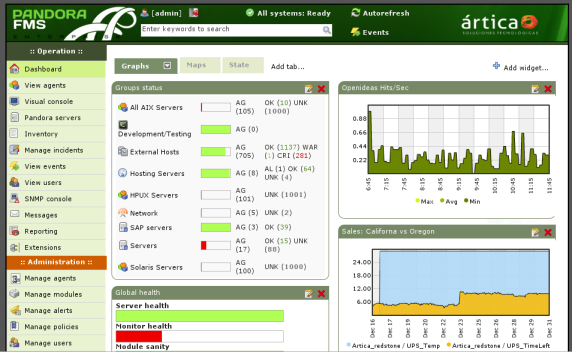
\includegraphics[width=10 cm]{images/pandoraFMS.png}}
\caption{Interfaz Pandora FMS}
\label{PandoraFMS}
\end{figure}


\item Zenoss (Zenoss Core)\cite{web-Zenoss} es una aplicación de informática de código abierto, plataforma para la gestión de red y servidores basada en el servidor de aplicaciones Zope. Zenoss Core provee una interfaz web que permite a los administradores de sistemas monitorear disponibilidad, inventario/configuración, desempeño y eventos.

\begin{figure}[hbtp]
\centerline{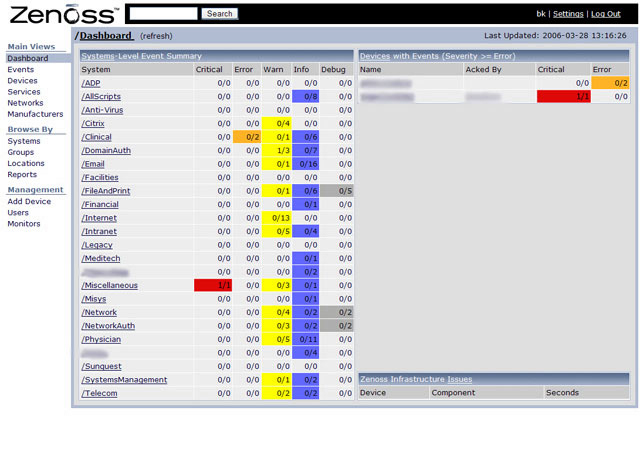
\includegraphics[width=10cm]{images/Zenossscreen.jpg}}
\caption{Interfaz Zenoss}
\label{Zenoss}
\end{figure}

\end{itemize}
    
    
\section{Funcionamiento de Nagios}

%%Explicación de cómo funciona Nagios

El funcionamiento básico de Nagios consiste en una arquitectura cliente-servidor mediante ejecución de polling periódico de chequeos de recursos (con agente) y servicios (sin agente) sobre sistemas cliente. Cuando se detecta un error la plataforma es capaz de enviar una notificación (sobre diferentes modos de comunicación) a los contactos administrativos, informando del estado del servicio que ha provocado el error, incluyendo informes de estado, de logs e históricos web).

Agentes Nagios

Una gran parte del monitoreo se puede hacer remotamente. Todo servicio publicado en la red, se puede monitorear sin necesidad de instalar nada en el host monitoreado. Sin embargo hay recursos que no se pueden monitorear remotamente, como por ejemplo:
\begin{itemize}

\item  espacio libre en disco
\item  memoria en uso
\item  carga de CPU
\item  servicios activos
\item  cantidad de usuarios logueados
Para ello es necesario instalar agentes. Estos agentes, mediante plugins, chequean el estado de los recursos y envían los datos al servidor Nagios. El tipo de conexión es pull, es decir, el servidor Nagios contacta cada cierto intervalo de tiempo a los agentes, les indica qué comandos ejecutar y obtiene los resultados.
Existen varios protocolos utilizados para la comunicación entre agentes y Nagios:
\item  NRPE Nagios Remote plugin Executor. Es el protocolo más utilizado y recomendado por Nagios. Se accede mediante el plugin check\_nrpe.
\item  NSCA Nagios Service Check Acceptor.
\item  NSCP: protocolo nativo de NSClient++
\item  NRDP: reemplazo NSCA.
\item  Syslog: protocolo estándar para transmisión de logs en Unix.
\item  SNMP: Simple Network Management Protocol. Protocolo estándar para administración y monitoreo de dispositivos de red.


\end{itemize}


%%Se pueden incluir figuras como por ejemplo la Figura~\ref{figura1} de la página \pageref{figura1}

%%\begin{figure}
%%\centerline{\includegraphics[width=6cm]{nagios3-1.png}}
%%\caption{Figura de ejemplo}
%%\label{figura1}
%%\end{figure}

Nagios sigue grosso modo la siguiente estructura:

Un núcleo de la aplicación que forma la lógica de control de negocio de la aplicación contiene el software necesario para realizar la monitorización de los servicios y máquinas de la red para la que está preparado. Hace uso de diversos componentes que vienen con la aplicación, y puede hacer uso de otros componentes realizados por terceras personas.
Aunque permite la captura de paquetes SNMP Trap para notificar sucesos, no es un sistema de monitorización y gestión basado en SNMP sino que realiza su labor basándose en una gran cantidad de pequeños módulos software que realizan chequeos de parte de la red.

Muestra los resultados de la monitorización y del uso de los diversos componentes en una interfaz web a través de un conjunto de CGI’s y de un conjunto de páginas HTML que vienen incorporadas de serie. Y que permiten al administrador una completa visión de qué ocurre, dónde y en algunos casos, por qué.
Por último, si se compila para ello, Nagios guardará los históricos en una base de datos para que al detener y reanudar el servicio de monitorización, todos los datos sigan como iban, sin cambios.


Así que en las siguientes páginas, antes de profundizar en el uso de Nagios, vamos a explicar cómo se realiza correctamente la instalación de este sistema, que no es nada trivial; al menos no es algo rápido.

\section{Instalación de Nagios}

En este apartado se explica cómo instalar Nagios de dos formas, desde repositorio y también compilando su código fuente. Ambos métodos tienen como distribución objetivo CentOs/RedHat.

\subsection{Instalación desde repositorio}

Suponiendo que se tiene acceso root a la máquina, el comando a ejecutar como superusuario es el siguiente

\begin{verbatim}
yum install nagios*
\end{verbatim}

esto se encargará de instalar Nagios, sus dependencias y los plugins. Los plugins nos permiten un mayor control de los sistemas a monitorizar así como una visualización más completa de la información.

\subsection{Instalación desde código fuente}

En primer lugar debemos crear el usuario y grupo al que pertenecerá la ejecución de Nagios. Esto se realiza con los siguientes comandos en modo superusuario

\begin{verbatim}
groupadd nagios
groupadd nagcmd
useradd nagios -g nagios
useradd nagios -g nagcmd
\end{verbatim}

El usuario Nagios será el que tendrá en ejecución el daemon correspondiente. Además hemos creado dos grupos, \textbf{nagios} y \textbf{nagcmd}

\begin{itemize}
\item \textbf{nagios}: El grupo principal de Nagios.
\item \textbf{nagcmd}: Este es el grupo que permite la ejecución de comandos externos a través de la interfaz web.
\end{itemize}

Ahora necesitamos instalar las dependencias, incluyendo el servidor web. De nuevo como superusuario ejecutamos lo siguiente

\begin{verbatim}
yum -y install httpd php glibc glibc-common gd gd-devel net-snmp
yum -y groupinstall "Development Tools"
\end{verbatim}

\textbf{httpd} y \textbf{php} serán los encargados del servidor web. \textbf{glibc}, \textbf{glibc-common}, \textbf{gd} y \textbf{gd-devel} son librerías para el manejo de gráficos y \textbf{net-snmp} es el que incluye las librerías para manejar el protocolo SNMP, que nos permitirá monitorizar los ordenadores en red.
\\

\textbf{Development Tools} instala todos los paquetes necesarios para poder compilar los códigos fuente. Incluye, como pequeño ejemplo, gcc y make.
\\

Ahora ya estamos listos para descargar el código fuente. En el momento de escribir esta memoria la última versión disponible es la 4.0.8 y es la que se usará a lo largo de la memoria, pero los pasos deberían ser iguales o muy similares en las versiones posteriores.
\\

En primer lugar, descargamos y descomprimimos las fuentes de Nagios Core. Nagios Core es el engine que tiene toda la lógica de la aplicación, sobre él se añadirán plugins y demás para personalizarlo.

\begin{verbatim}
wget http://netcologne.dl.sourceforge.net/project/nagios/
            nagios-4.x/nagios-4.0.8/nagios-4.0.8.tar.gz
tar -xzf nagios-4.0.8.tar.gz
\end{verbatim}

Accedemos a la carpeta y realizamos un \textbf{./configure}

\begin{verbatim}
cd nagios-4.0.8
./configure
\end{verbatim}

\textbf{./configure} comprueba que las dependencias del programa estén satisfechas (por lo menos las esenciales). En caso de no cumplirse algún requisito indispensable el programa saldrá con un mensaje de error indicando qué se debe instalar. Si el programa considera que se cumplen los requisitos mínimos generará un fichero \textbf{Makefile} con los comandos necesarios para compilar e instalar el programa.
\\

Una vez el comando ha acabado ejecutamos

\begin{verbatim}
make all
make install
make install-init
make install-commandmode
make install-config
make install-webconf
\end{verbatim}

\begin{itemize}
\item \textbf{all}: Compila el programa dejando los ejecutables preparados para ejecutarse desde local o para instalarse.
\item \textbf{install}: Copia los ejecutables base a sus respectivas carpetas para que se puedan encontrar desde el \$PATH.
\item \textbf{install-init}: Este comando instala el fichero en /etc/rc.d/init.d para poder iniciarlo y pararlo de manera cómoda.
\item \textbf{install-commandmode}: Instala y configura los permisos en el directorio para almacenar los ficheros externos de comandos.
\item \textbf{install-config}: Este comando instala plantillas de configuración en /usr/local/nagios/etc para que sea más fácil su edición.
\item \textbf{install-webconf}: Instala el fichero de configuración de Apache.
\end{itemize}

Ahora vamos a compilar e instalar los plugins desde código fuente, a fecha de escribir este artículo la última versión de los plugins es la 2.0.3

\begin{verbatim}
wget http://nagios-plugins.org/download/nagios-plugins-2.0.3.tar.gz
tar -xzf nagios-plugins-2.0.3.tar.gz
cd nagios-plugins-2.0.3
\end{verbatim}

Una vez descargados procedemos a su configuración, compilación e instalación.

\begin{verbatim}
./configure
make
make install
\end{verbatim}

Con esto tendríamos instalado Nagios y sus plugins desde código fuente, ahora sólo queda configurarlos. Esto se explica más adelante.

\section{Configuración}

\subsection{Configuración de Nagios}
En esta sección se explica cómo configurar Nagios paso a paso.
\\

En primer lugar debemos crear los usuarios. En esta memoria crearemos un usuario administrador y otro que sólo pueda consultar la interfaz web.

\begin{verbatim}
htpasswd -c /usr/local/nagios/etc/htpasswd.users administrador
htpasswd /usr/local/nagios/etc/htpasswd.users usuario
\end{verbatim}

En ambos casos se pedirá que se introduzca una contraseña, en nuestro ejemplo serán \textbf{labora2000} y \textbf{practicas} respectivamente. El parámetro -c usado en el primer comando crea el fichero si no existe, de existir lo sobreescribe.
\\

El siguiente paso es cambiar el e-mail de contacto. Este e-mail será el que recibirá todas las notificaciones de Nagios. Para ello editamos el fichero /usr/local/nagios/etc/objects/contacts.cfg y cambiamos la siguiente línea para que contenga nuestro e-mail

\begin{verbatim}
email  usuario@gmail.com; <<***** CHANGE THIS TO YOUR EMAIL ADDRESS ******
\end{verbatim}

Ahora debemos decirle a Apache que carge el módulo PHP o la web no funcionará correctamente. Para ello modificamos el fichero /etc/httpd/conf/httpd.conf y añadimos la línea

\begin{verbatim}
LoadModule php5_module modules/libphp5.so
\end{verbatim}

con esto nos aseguramos de que funcione PHP en nuestro servidor web.
\\

Por último configuramos los usuarios de Nagios. Para ello hay que editar el fichero /usr/local/nagios/etc/cgi.cfg
\\

Hay que editar las líneas siguientes para incluir los usuarios que hemos creado

\begin{verbatim}
authorized_for_system_information=administrador,usuario
authorized_for_configuration_information=administrador
authorized_for_system_commands=administrador
authorized_for_all_services=administrador,usuario
authorized_for_all_hosts=administrador,usuario
authorized_for_all_service_commands=administrador
authorized_for_all_host_commands=administrador
\end{verbatim}

Las líneas hacen lo siguiente:

\begin{itemize}
\item \textbf{authorized\_for\_system\_information}: Estos usuarios podrán ver los procesos e información de los sistemas en la interfaz web.
\item \textbf{authorized\_for\_configuration\_information}: Estos usuarios podrán ver los comandos y la configuración de los sistemas a través de la interfaz web.
\item \textbf{authorized\_for\_system\_commands}: Estos usuarios podrán apagar y reiniciar Nagios.
\item \textbf{authorized\_for\_all\_services}: Estos usuarios podrán ver la información de todos los servicios monitorizados.
\item \textbf{authorized\_for\_all\_hosts}: Estos ususarios podrán ver la información de todos los sistemas monitorizados.
\item \textbf{authorized\_for\_all\_service\_commands}: Estos usuarios podrán ejecutar comandos sobre todos los servicios.
\item \textbf{authorized\_for\_all\_host\_commands}: Estos usuarios podrán ejecutar comandos sobre todos los sistemas.
\end{itemize}

De esta manera sólo le damos poderes totales al usuario \textbf{administrador} y poderes de consulta al usuario \textbf{usuario}.
\\

Con esto hemos acabado la configuración de Nagios, pero no es muy útil si no añadimos algunos hosts externos para monitorizar.

\subsection{Configuración de los hosts externos}

Para comenzar la configuración, crearemos el fichero /usr/local/nagios/etc/objects/hosts.cfg que contendrá todos los parámetros, hosts y servicios a configurar.
\\

La plantilla básica que vamos a usar para configurar cada uno de los hosts es la siguiente

\begin{verbatim}
define host {

    host_name                PC_108
    alias                    108 lab
    address                  150.128.49.108
    check_command            check-host-alive
    max_check_attempts       3
    check_period             24x7
    notification_intervaL    180
    notification_period      24x7
    notification_optionS     d,r,u

}
\end{verbatim}

\begin{itemize}
\item \textbf{host\_name}: Un nombre corto y único para identificar el ordenador.
\item \textbf{alias}: Un nombre largo o descripción para identificar el ordenador.
\item \textbf{address}: La dirección IP
\item \textbf{check\_command}: Comando que se ejecutará para saber si el host está disponible o no.
\item \textbf{max\_check\_attempts}: El número de intentos que realizará Nagios para comprobar si un host no está disponible después de que este no le responda.
\item \textbf{check\_period}: Indica el intervalo sobre el cual se puede hacer checks sobre el servidor.
\item \textbf{notification\_interval}: El intervalo que tardará Nagios en decirnos que el host todavía no está disponible.
\item \textbf{notification\_period}: Indica el intervalo sobre el cual se pueden enviar notificaciones a los usuarios.
\item \textbf{notification\_options}: Indica cuándo enviar notificaciones. \textbf{d}: Indicar cuando el host no está disponible. \textbf{u}: Indicar cuándo el host no es accesible. \textbf{r}: Indicar cuándo se ha recuperado el servidor.
\end{itemize}

Tendremos un bloque como el anterior \textbf{para cada uno} de los hosts que pretendemos monitorizar.
\\

El siguiente paso es el de configurar grupos, de manera que se pueda asignar la monitorización de un servicio al grupo entero en lugar de ir host por host. La plantilla es la siguiente

\begin{verbatim}
define hostgroup {

    hostgroup_name    grupolab1
    alias             Grupo laboratorio
    members           PC_108, PC_107, PC_105

}
\end{verbatim}

\begin{itemize}
\item \textbf{hostgroup\_name}: Nombre por el que se identifica el grupo.
\item \textbf{alias}: Pequeña descripción del grupo.
\item \textbf{members}: Hosts por nombre que pertenecen al grupo.
\end{itemize}

Y por último la plantilla usada para definir los servicios que queremos monitorizar es la siguiente
\begin{verbatim}
define service{

    hostgroup_name          grupolab1
    service_description     SSH
    check_period            24x7
    max_check_attempts      4
    contact_groups          admins
    notification_options    w,u,c,r
    notification_interval   960
    notification_period     24x7
    check_command           check_ssh
    
}
\end{verbatim}

\begin{itemize}
\item \textbf{hostgroup\_name}: El grupo o grupos a los que se le aplicará este servicio.
\item \textbf{service\_description}: Una pequeña descripción del servicio.
\item \textbf{check\_period}: Indica el intervalo sobre el cual se puede hacer checks sobre el servicio.
\item \textbf{max\_check\_attempts}: El número de intentos que realizará Nagios para comprobar si un servicio no está disponible después de que este no le responda.
\item \textbf{contact\_groups}: A qué grupo hay que enviarle las notificaciones.
\item \textbf{notification\_options}: Indica bajo qué condiciones se envían notificaciones. \textbf{w}: Cuando está en WARNING. \textbf{u}: Cuando está en UNKNOWN. \textbf{c}: Cuando está en CRITICAL. \textbf{r}: Cuando se ha recuperado.
\item \textbf{notification\_interval}: El intervalo que tardará Nagios en decirnos que el servicio todavía no está disponible.
\item \textbf{notification\_period}: Indica el intervalo sobre el cual se pueden enviar notificaciones a los usuarios.
\item \textbf{check\_command}: El comando que se ejecutará en este servicio.
\end{itemize}

El ejemplo anterior monitoriza el estado del servicio SSH en el grupo grupolab1.
\\

Ahora queda decirle a Nagios que lea el fichero que acabamos de crear, para ello hay que editar el fichero /usr/local/nagios/etc/nagios.cfg y hay que añadir la línea

\begin{verbatim}
cfg_file=/usr/local/nagios/etc/objects/hosts.cfg
\end{verbatim}

Ahora sólo queda reiniciar los servicios y todo estará funcionando.

\begin{verbatim}
service httpd restart
service nagios restart
\end{verbatim}

\section{Acceso a Nagios mediante el navegador}

Para acceder a la interfaz web de Nagios una vez seguidos los pasos anteriores, no hay más que ir a \url{http://localhost/nagios/}.

La página principal es la siguiente

\begin{figure}[h!]
  \centering
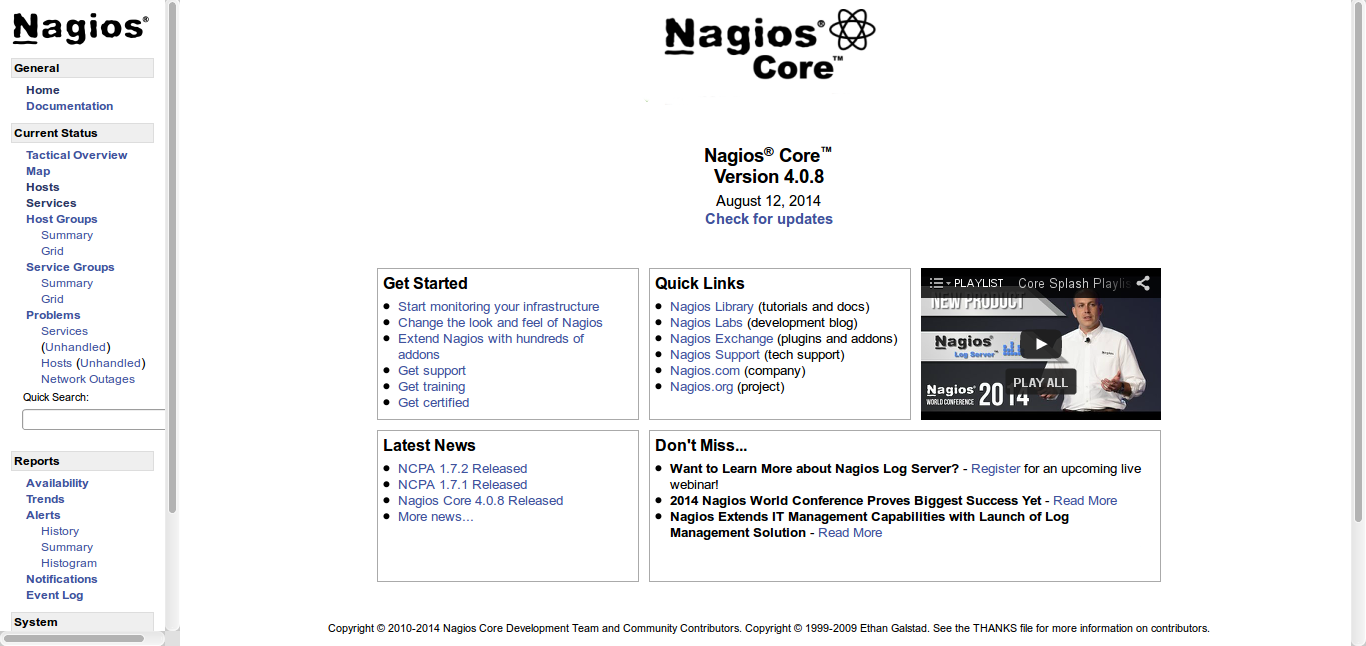
\includegraphics[width=10cm]{images/0.png} 
  \caption{Página principal.}
\end{figure}

Se debe explicar cómo se debe configurar el servidor web para acceder a Nagios a través del navegador
y  también la interfaz web que presenta Nagios.

\section{Experiencia de instalación y configuración de Nagios}

Se deben detallar los pasos que se han seguido para la instalación y configuración de Nagios
tanto para monitorizar el sistema local como sistemas remotos.

\begin{thebibliography}{1}

\bibitem{web} Página web del proyecto de Nagios: \url{http://www.nagios.org}
\bibitem{nagios-wikipedia} Wikipedia Nagios: \url{http://es.wikipedia.org/wiki/Nagios}
\bibitem{web-PandoraFMS} Página web del proyecto de PandoraFMS: \url{http://pandorafms.com/}
\bibitem{web-Zenoss} Página web del proyecto de Zenoss: \url{http://www.zenoss.com/}
\end{thebibliography}

\end{document}
